\chapter{Requirement Elicitation}

\section{Use Cases}

In this chapter, we will look at four main use cases of SQAT. We do not cover all possible use cases because we want to focus on the use cases that are relevant when setting up the foundation of SQAT. The seven main uses cases are, submitting source code for testing, submitting source code for assignment, creating new assignment for submission, checking results of all students, checking assignment results, set up SQAT continuous integration and perform quality assessment request from GitHub webhook. The use case diagram for SQAT is shown in Figure \ref{figure:SQAT_use_case_diagram}. 

\begin{figure}[t]
    \centering
    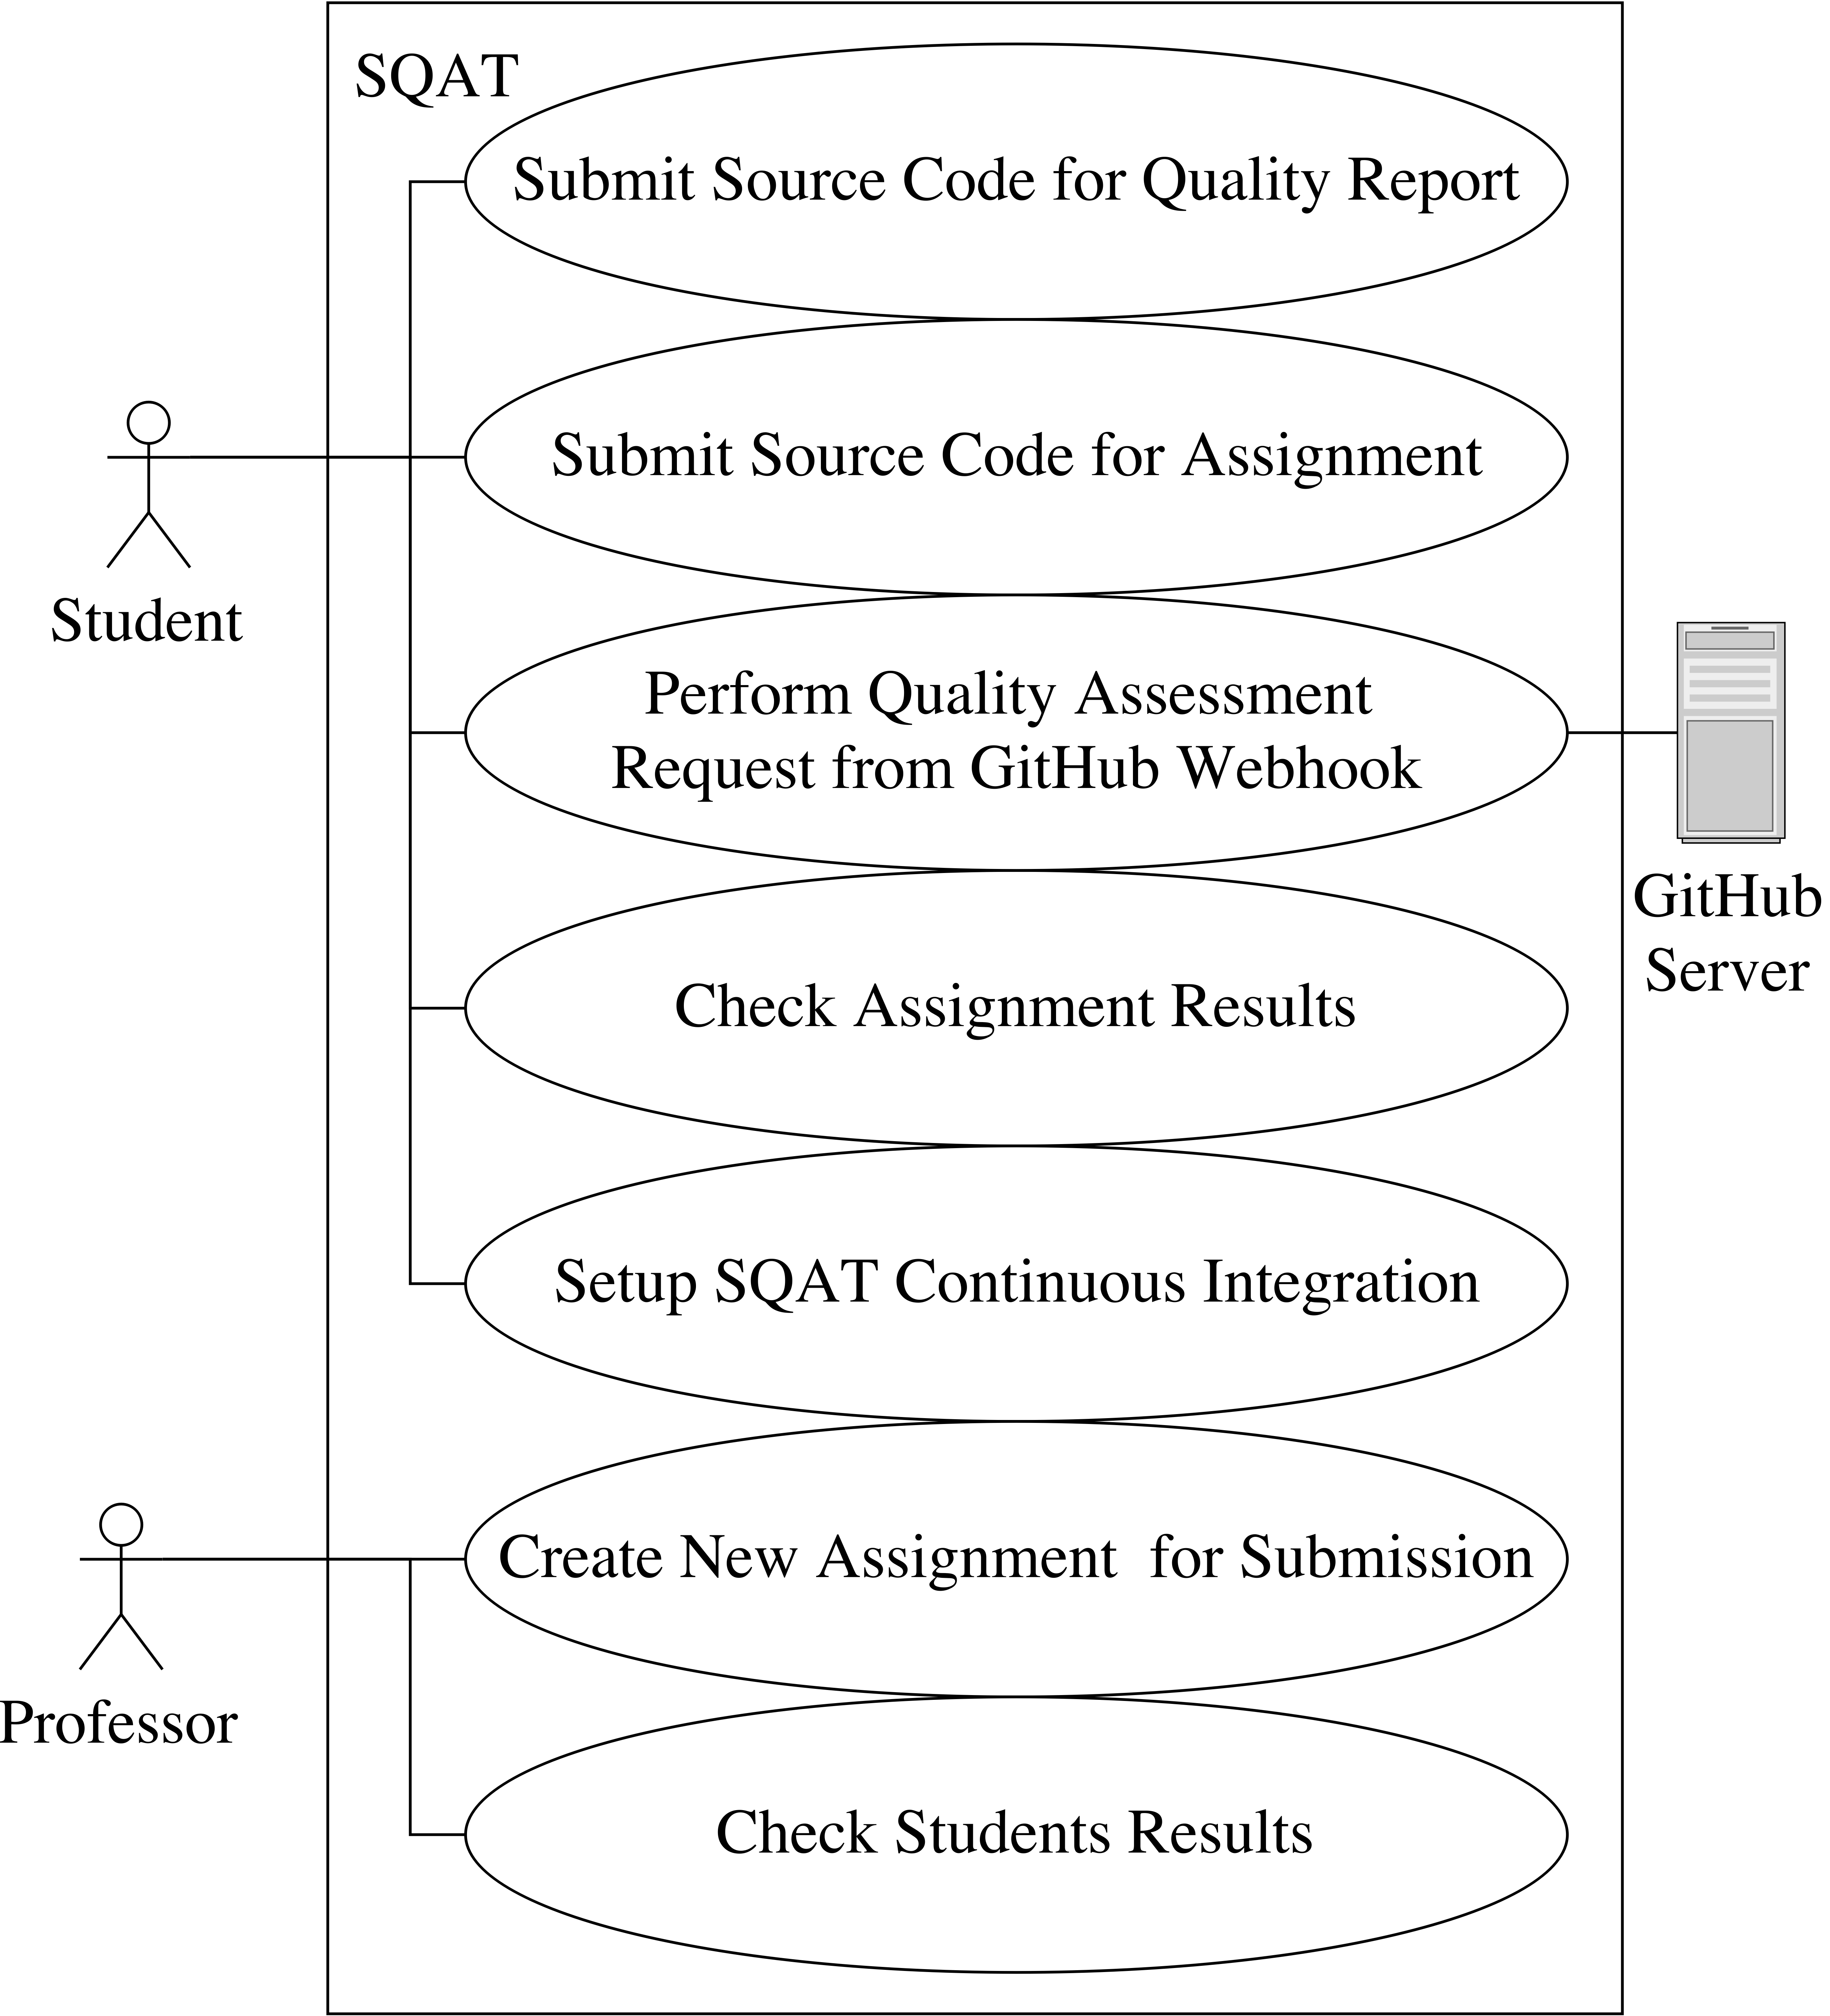
\includegraphics[width=12cm]{SQAT_use_case_diagram.png}
    \caption{SQAT use case diagram}
    \label{figure:SQAT_use_case_diagram}
\end{figure}

\usecases
    {Submit Source Code for Quality Report}
    {Student}
    {Student submits source code so that SQAT can assess the source code. }
    {
        1. Student accesses SQAT website\\
        2. Student uploads compressed source codes\\
        3. SQAT Server decompressed the source codes\\
        4. SQAT Server analyses the codes\\
        5. SQAT generates overall quality report for student\\
        5. Student receive the quality report through the website
    }
    
\usecases
    {Submit Source Code for Assignment}
    {Student}
    {Student submits source code for their assignment. }
    {
        1. Student accesses SQAT website\\
        2. Student sign in using NTU account\\
        3. Student select assignment to be completed\\
        4. Student uploads compressed source codes\\
        5. SQAT Server puts a new request of job queue\\
        6. SQAT Server sends an email to students once the job done\\
        7. Student is informed that the server is processing the request\\
        8. Student will be notified through NTU email
    }
    
\usecases
    {Create New Assignment for Submission}
    {Professor}
    {Professor creates a new assignment for students to submit their assignments. }
    {
        1. Professor accesses SQAT website\\
        2. Professor sign in using NTU account\\
        3. Professor will create a new assignment by inputting:\\
        \ \ \ \ a. Assignment name\\
        \ \ \ \ b. Assignment deadline\\
        \ \ \ \ c. Course for the assignment\\
        4. SQAT Server creates a new assignment
    }
    
\usecases
    {Check Student Results}
    {Professor}
    {Professor checks all student results for an assignment after the deadline. }
    {
        1. Professor accesses SQAT website\\
        2. Professor sign in using NTU account\\
        3. Professor selects the assignment that he want to check\\
        4. SQAT Server generates a report with all results
    }

\usecases
    {Check Assignment Results}
    {Student}
    {Student checks assignment result after the assignment is assessed by SQAT}
    {
        1. Student accesses SQAT website\\
        2. Student sign in using NTU account\\
        3. Student selects the assignment that he want to check\\
        4. SQAT Server retrieves results from database.\\
        5. Student evaluate the results in the website
    }

\usecases
    {Set up SQAT Continuous Integration}
    {Student}
    {Student wants to set up continuous integration so that SQAT will check source codes hosted in GitHub automatically when new source codes are checked in to the repository}
    {
        1. Student accesses SQAT website\\
        2. Student sign in using NTU account\\
        3. Student selects SQAT continuous integration\\
        4. The website shows instruction to setup GitHub webhook \\
        5. Student setup continuous integration in GitHub\\
        6. SQAT Server tests if the webhook is setup correctly\\
        7. Student continues his/her assignment/development
    }

\usecases
    {Perform Quality Assessment Request from GitHub Webhook}
    {GitHub Server}
    {GitHub Server informs SQAT to perform quality assessment. }
    {
        1. GitHub Server receives a code commit from student\\
        2. GitHub Server informs SQAT Server about the event\\
        3. SQAT receives the notification\\
        4. SQAT Server downloads the latest source codes\\
        5. SQAT Server performs quality assessment on the source code\\
        6. SQAT Server tests if the webhook is setup correctly\\
        7. SQAT Server sends a report via email to students
    }

\section{Hardware and Software Requirements}

The hardware requirement for SQAT server is a computer with 1 CPU core, 1GB RAM, 20GB persistent storage. SQAT server codes must be able to run in any operating system with Docker installed \footnote{Docker Toolbox can be installed at https://www.docker.com/docker-toolbox}. 